\documentclass[11pt]{beamer}
\usetheme{Dresden}
\usepackage[utf8]{inputenc}
\usepackage{amsmath}
\usepackage{amsfonts}
\usepackage{amssymb}
\usepackage{tikz}
\usepackage{graphicx}
\usepackage[backend=bibtex]{biblatex}
\addbibresource{talkslides.bib}

\newcommand{\vrcomplex}[2][0.5]{
\begin{center}
\begin{tikzpicture}[scale=#1]
  \coordinate (a) at (2,3.3);
  \coordinate (b) at (7,4);
  \coordinate (c) at (0,0);
  \coordinate (d) at (3.5,0);

\clip (-3, -3) rectangle (10, 7);
\draw[white, fill, opacity=0] (-3, -3) rectangle (10, 7);

  \draw[black,fill] (a) circle [radius=0.1cm];
  \draw[black,fill] (b) circle [radius=0.1cm];
  \draw[black,fill] (c) circle [radius=0.1cm];
  \draw[black,fill] (d) circle [radius=0.1cm];

\draw[cyan, fill, opacity= 0.3] (a) circle (#2cm);
\draw[black] (a) circle (#2cm);
\draw[cyan, fill, opacity= 0.3] (b) circle (#2cm);
\draw[black] (b) circle (#2cm);
\draw[cyan, fill, opacity= 0.3] (c) circle (#2cm);
\draw[black] (c) circle (#2cm);
\draw[cyan, fill, opacity= 0.3] (d) circle (#2cm);
\draw[black] (d) circle (#2cm);
\end{tikzpicture}
\end{center}
}

\newcommand{\annuluscomplex}[1]{
\begin{figure}
\noindent\makebox[\textwidth]{%
\begin{tikzpicture}[scale=0.3]
%\begin{tikzpicture}[remember picture, overlay, scale=0.3]
%\tikzset{shift={(current page.center)},yshift=0cm}
\clip (-20, -10) rectangle (20, 10);
\draw[white, fill, opacity=0] (-20, -10) rectangle (20, 10);

\def\points{8.092593/0.134148,8.447231/0.949326,7.658496/1.144397,8.815373/2.177150,8.398666/2.076670,
9.006517/3.977381,7.520945/2.129330,6.698849/2.255754,5.807683/2.718666,7.062904/3.015901,
7.278569/4.457003,5.898714/4.987420,4.562342/5.118081,4.727490/6.667248,4.005391/6.592861,
3.983471/7.332549,4.038059/8.096364,3.859597/8.469849,3.195593/6.353141,3.981205/6.389805,
2.429519/8.228017,3.216939/6.555953,1.802313/7.954675,2.259787/8.041740,-0.397224/9.074358,
0.401439/7.953553,-1.266806/7.655207,-0.623094/8.432865,-1.053032/8.554193,-3.427812/7.770895,
-3.352173/7.103145,-3.918641/6.328826,-3.049035/7.426226,-2.966824/6.214639,-4.897973/5.293921,
-4.003319/7.130895,-4.712890/5.274353,-7.091653/5.528760,-5.655604/5.897540,-6.628111/4.522957,
-5.341439/5.245499,-8.360414/3.793542,-7.223336/4.216060,-7.555821/3.819587,-7.634792/2.563077,
-6.865465/0.812593,-8.336023/1.255058,-7.045293/1.036940,-8.049704/0.071260,-9.388684/-0.655015,
-8.968349/0.711340,-7.298501/-0.970684,-7.979053/-0.100698,-8.845275/-2.088935,-8.152570/-1.446517,
-7.195373/-3.045787,-8.253632/-2.281902,-6.395403/-2.900581,-7.635319/-4.477232,-5.337140/-5.388422,
-6.981240/-4.074050,-5.165616/-3.986240,-6.545813/-6.218857,-5.876391/-5.532203,-6.071537/-6.550160,
-4.202732/-5.660057,-3.449910/-6.121640,-3.412754/-8.166190,-3.313574/-6.292893,-2.183215/-6.090390,
-1.688938/-7.667467,-1.101403/-6.677577,-0.731159/-7.654493,0.701523/-9.010581,-1.000123/-8.899405,
1.008500/-8.270074,0.095397/-7.204591,0.247374/-6.901711,2.207983/-6.904603,2.225776/-8.183645,
2.731266/-7.370991,3.809154/-8.507204,4.589025/-8.216510,3.768458/-7.888926,5.126484/-5.980651,
4.792897/-6.223641,6.453863/-6.807602,6.788623/-5.535615,5.397679/-6.199476,6.782544/-6.078341,
6.976776/-3.272989,7.113013/-3.707895,8.333235/-2.149533,6.721281/-2.383298,7.054791/-2.247895,
6.601233/-1.062992,9.174918/-0.376968,8.372294/0.453995,7.922283/-2.005824,8.417951/1.096316}

\foreach \x / \y in \points{
\draw[cyan, fill, opacity=0.3] (\x,\y) circle (#1cm);
}

\foreach \x / \y in \points{
\draw[gray] (\x,\y) circle (#1cm);
}

\foreach \x / \y in \points{
\draw[black,fill] (\x,\y) circle [radius=0.1cm];
}
\end{tikzpicture}
}
\end{figure}
}

\author{Mitchell Riley \\ Supervisor: Ben Burton}
\title{Persistence Modules and Stability}
\date{17th October 2014}
\beamertemplatenavigationsymbolsempty
\setbeamertemplate{footline}{}
\begin{document}

\begin{frame}
\titlepage
\end{frame}

\section{Persistent Homology}

\begin{frame}
\frametitle{Singular Homology}
Choose a dimension $n$, then
\begin{align*}
H_n(-) &: \mathbf{Top} \to \mathbf{Ab}
\end{align*}
describes the $n$-dimensional `holes'.
\end{frame}

\begin{frame}
\begin{columns}[c]
\column{.3\textwidth}
\begin{center}

\begin{tikzpicture}[scale=1]
\draw (1, 1) circle (1cm);
\end{tikzpicture}
\end{center}
\begin{align*}
  H_0(\mathbb{S}^1) &= \mathbb{Z} \\
  H_1(\mathbb{S}^1) &= \mathbb{Z} \\
  H_2(\mathbb{S}^1) &= \{1\}
\end{align*}
\uncover<2->{\column{.3\textwidth}
\begin{center}
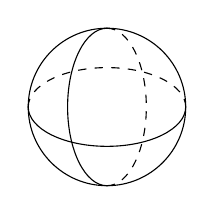
\begin{tikzpicture}[scale=1]
    \draw (-1,0) arc (180:360:1cm and 0.5cm);
    \draw[dashed] (-1,0) arc (180:0:1cm and 0.5cm);
    \draw (0,1) arc (90:270:0.5cm and 1cm);
    \draw[dashed] (0,1) arc (90:-90:0.5cm and 1cm);
    \draw (0,0) circle (1cm);
\end{tikzpicture}
\end{center}
\begin{align*}
  H_0(\mathbb{S}^2) &= \mathbb{Z} \\
  H_1(\mathbb{S}^2) &= \{1\} \\
  H_2(\mathbb{S}^2) &= \mathbb{Z}
\end{align*}
}
\uncover<3->{\column{.3\textwidth}
\begin{center}
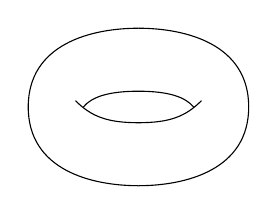
\begin{tikzpicture}[scale=0.4]
\draw (-3.5,0) .. controls (-3.5,2) and (-1.5,2.5) .. (0,2.5);
\draw[xscale=-1] (-3.5,0) .. controls (-3.5,2) and (-1.5,2.5) .. (0,2.5);
\draw[rotate=180] (-3.5,0) .. controls (-3.5,2) and (-1.5,2.5) .. (0,2.5);
\draw[yscale=-1] (-3.5,0) .. controls (-3.5,2) and (-1.5,2.5) .. (0,2.5);

\draw (-2,.2) .. controls (-1.5,-0.3) and (-1,-0.5) .. (0,-.5) .. controls (1,-0.5) and (1.5,-0.3) .. (2,0.2);

\draw (-1.75,0) .. controls (-1.5,0.3) and (-1,0.5) .. (0,.5) .. controls (1,0.5) and (1.5,0.3) .. (1.75,0);
\end{tikzpicture}
\end{center}
\begin{align*}
  H_0(\mathbb{T}^2) &= \mathbb{Z} \\
  H_1(\mathbb{T}^2) &= \mathbb{Z} \oplus \mathbb{Z} \\
  H_2(\mathbb{T}^2) &= \mathbb{Z}
\end{align*}
}
\end{columns}
\end{frame}

\begin{frame}
\frametitle{Singular Homology}
\begin{theorem}
A continuous map $f : X \to Y$ induces a homomorphism $f_* : H_k(X) \to H_k(Y)$ for all $k$.
\end{theorem}
\end{frame}

\begin{frame}
\frametitle{Singular Homology}
\begin{align*}
H_n(-) &: \mathbf{Top} \to \mathbf{Ab}\\
\uncover<2->{H_n(-; R) &: \mathbf{Top} \to R\textrm{-}\mathbf{Mod}} \\
\uncover<3->{H_n(-; \mathbf{k}) &: \mathbf{Top} \to \mathbf{Vect_k}} \\
\end{align*}
\end{frame}

\begin{frame}
\annuluscomplex{0}
\end{frame}

\begin{frame}
\frametitle{$r=2$}
\annuluscomplex{2}
\begin{align*}
  H_0(X) &= \mathbb{Z} \\
  H_1(X) &= \mathbb{Z}
\end{align*}
\end{frame}

\begin{frame}
\frametitle{$r=0.3$}
\annuluscomplex{0.3}
\begin{align*}
  H_0(X) &= \mathbb{Z}^{73} \\
  H_1(X) &= \{1\}
\end{align*}
\end{frame}

\begin{frame}
\frametitle{$r=10$}
\annuluscomplex{10}
\begin{align*}
  H_0(X) &= \mathbb{Z} \\
  H_1(X) &= \{1\}
\end{align*}
\end{frame}

\begin{frame}
\annuluscomplex{0.3}
\begin{align*}
X_{1} \invisible{\subset X_{2} \subset X_{3} \subset X_{4} \subset X_{5}}
\end{align*}
\end{frame}
\begin{frame}
\annuluscomplex{0.6}
\begin{align*}
X_{1} \subset X_{2} \invisible{\subset X_{3} \subset X_{4} \subset X_{5}}
\end{align*}
\end{frame}
\begin{frame}
\annuluscomplex{1}
\begin{align*}
X_{1} \subset X_{2} \subset X_{3} \invisible{\subset X_{4} \subset X_{5}}
\end{align*}
\end{frame}
\begin{frame}
\annuluscomplex{4}
\begin{align*}
X_{1} \subset X_{2} \subset X_{3} \subset X_{4} \invisible{\subset X_{5}}
\end{align*}
\end{frame}
\begin{frame}
\annuluscomplex{8}
\begin{align*}
X_{1} \subset X_{2} \subset X_{3} \subset X_{4} \subset X_{5}
\end{align*}
\end{frame}

\begin{frame}
We have a filtration:
\begin{align*}
X_{1} \subset X_{2} \subset X_{3} \subset X_{4} \subset X_{5}
\end{align*}

This gives us a diagram of spaces with inclusion maps:
\begin{align*}
X_{1} \to X_{2} \to X_{3} \to X_{4} \to X_{5}
\end{align*}

Now find the homology of each space, giving a diagram of groups and homomorphisms:
\begin{align*}
H(X_{1}) \to H(X_{2}) \to H(X_{3}) \to H(X_{4}) \to H(X_{5})
\end{align*}
\end{frame}

\begin{frame}
\frametitle{Zomorodian and Carlsson (2005)}
If the ground ring is a field $\mathbf{k}$, we have a diagram of $\mathbf{k}$-vector spaces.

\begin{theorem}
Any finite diagram of finite dimensional vector spaces decomposes into a sum of intervals.
\end{theorem}
\end{frame}

\begin{frame}
\frametitle{Zomorodian and Carlsson (2005)}
\begin{gather*}
H_0(X_{1}) \to H_0(X_{2}) \to H_0(X_{3}) \to H_0(X_{4}) \to H_0(X_{5}) \\
\parallel \\ \mathbf{k} \to \mathbf{k} \to \mathbf{k} \to \mathbf{k} \to \mathbf{k} \\[1px]
\oplus \\ \mathbf{k} \to \mathbf{k} \to 0 \to 0 \to 0 \\
\oplus \\ \mathbf{k} \to 0 \to 0 \to 0 \to 0 \\
\oplus \\ \mathbf{k} \to 0 \to 0 \to 0 \to 0 \\
\vdots \\
\uncover<2->{\mathcal{B}_0 = \{[1, 5], [1, 3), [1, 2), [1, 2), \dots \}}
\end{gather*}

\end{frame}

\begin{frame}
\frametitle{Zomorodian and Carlsson (2005)}
\begin{gather*}
H_1(X_{1}) \to H_1(X_{2}) \to H_1(X_{3}) \to H_1(X_{4}) \to H_1(X_{5}) \\
\parallel \\ 0 \to \mathbf{k} \to \mathbf{k} \to \mathbf{k} \to 0 \\
\oplus \\ 0 \to \mathbf{k} \to 0 \to 0 \to 0 \\
\oplus \\ 0 \to 0 \to \mathbf{k} \to 0 \to 0 \\
\vdots
\end{gather*}

\begin{align*}
\mathcal{B}_1 = \{[2,5), [2,3), [2,3), \dots \}
\end{align*}
\end{frame}

\begin{frame}
\frametitle{Zomorodian and Carlsson (2005)}
\begin{definition}
A \emph{barcode} (or \emph{persistence diagram}) is a multiset of points in the half plane
\begin{align*}
\mathcal{H} = \{ (p, q) \in \mathbb{R}^2 : p < q \}
\end{align*}
\end{definition}
\pause
\begin{center}
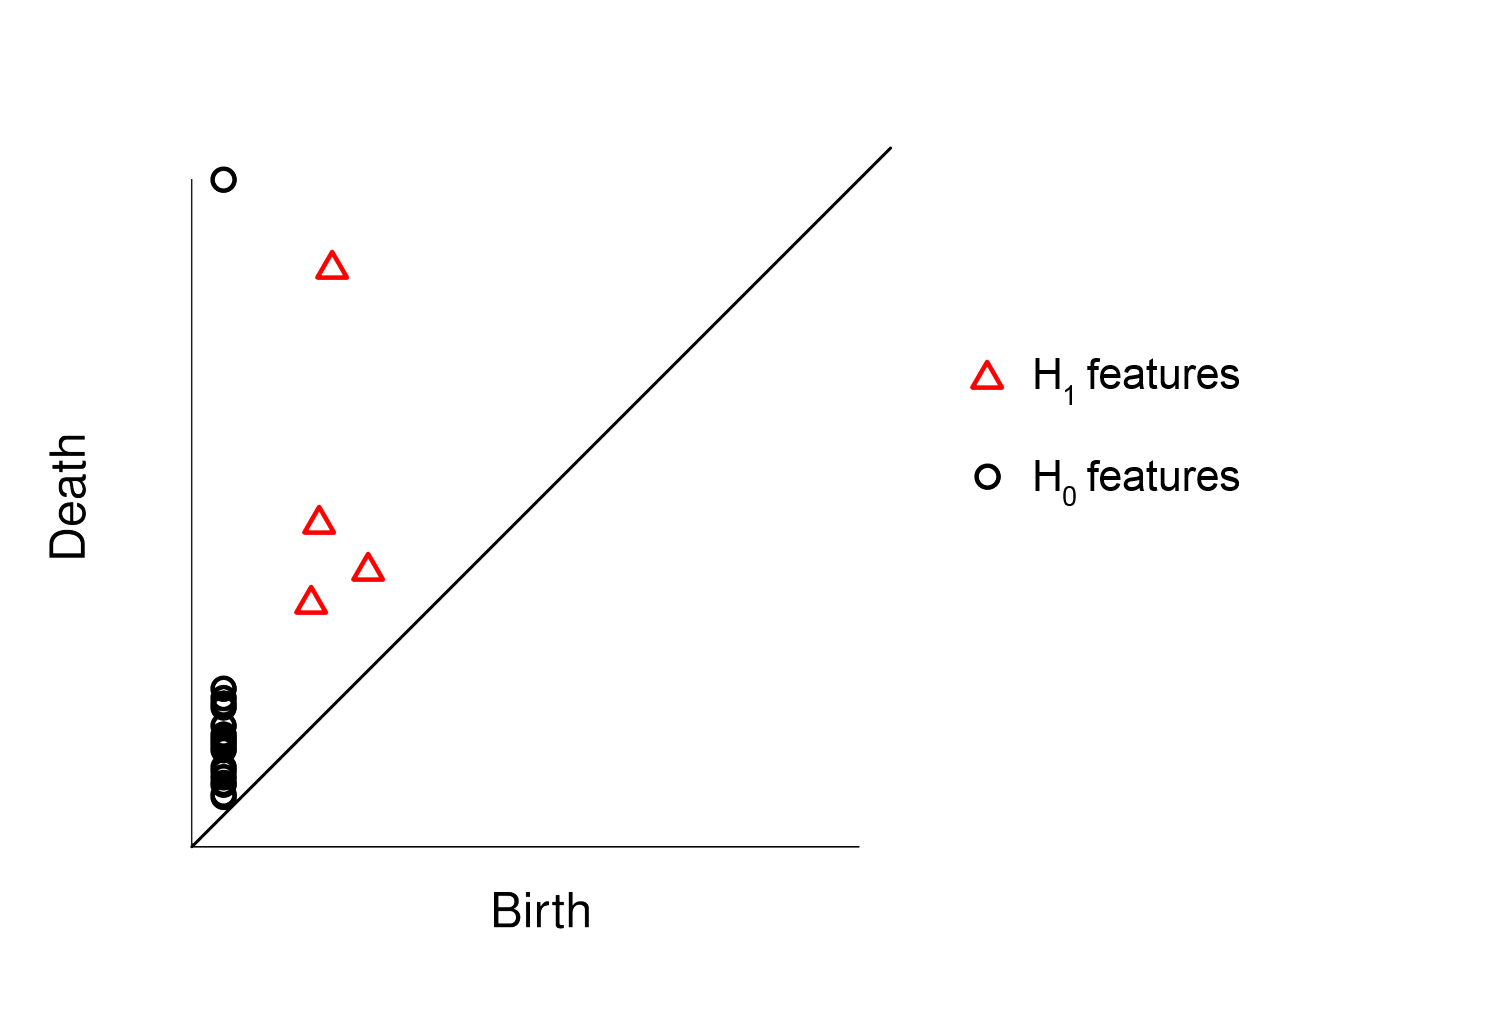
\includegraphics[width=\textwidth,height=0.6\textheight,keepaspectratio]{diagram.png}
\end{center}
\end{frame}

\begin{frame}
\frametitle{The Story So Far}
\belowdisplayskip=3pt
\abovedisplayskip=3pt
\begin{itemize}[<+->]
\item Begin with a data set $K \subset \mathbb{R}^n$
\begin{align*}
K = \{(0.125, 0.72), (0.627, 0.92), \dots \}
\end{align*}
\item Construct a filtration $\{X_i\}$
\begin{align*}
X_1 \subseteq X_2 \subseteq \dots
\end{align*}
\item Calculate homology of each space
\begin{align*}
H(X_1) \to H(X_2) \to \dots
\end{align*}
\item Determine the barcode of this diagram of vector spaces
\begin{align*}
\mathcal{B} = \{[0, 3), [2, 5), \dots\}
\end{align*}
\item Find features with long intervals
\end{itemize}
\end{frame}

\begin{frame}
\frametitle{Applications}
\begin{itemize}
\item Analysis of treatment response in breast cancer patients (DeWoskin et al, 2010)
\item Natural language processing (Zhu, 2013)
\item Computer vision (Lamar-Le\'{o}n et al, 2012)
\end{itemize}
\end{frame}

\section{Persistence Modules}

\begin{frame}
\frametitle{Persistence modules}
\begin{definition}
A \emph{persistence module} $\mathbb{V}$ over a poset $P$ is a collection of vector spaces $\{V_i\}_{i \in P}$ and linear maps $\{v_s^t : V_s \to V_t\}_{s \leq t}$ such that
\begin{align*}
v_r^t = v_s^t \circ v_r^s \text{ for all } r \leq s \leq t
\end{align*}
\end{definition}
Here we are interested in persistence modules over the real numbers $\mathbb{R}$.
\end{frame}

\begin{frame}
\frametitle{Sublevel persistence modules}
Let $f : X \to \mathbb{R}$ be a function and define $X_a = f^{-1}((-\infty, a])$.
\\~\\
This gives us a filtration $\{X_a\}_{a \in \mathbb{R}}$, and therefore a persistence module $\mathbb{V}$ with
\begin{align*}
V_t &= H(X_t)\\
v_s^t &= \eta_s^t
\end{align*}

The spaces we created above can be defined this way. Let $X = \mathbb{R}^n$, and $f(x) = \text{distance from $x$ to closest point in $K$}$.
\end{frame}

\begin{frame}
\frametitle{Persistence modules can be wild!}
\begin{example}[Crawley-Boevey, 2012]
Consider the persistence module:
\begin{align*}
\mathbb{V} = \prod_{n=1}^\infty \mathbb{I}[0, \tfrac{1}{n}]
\end{align*}
$\mathbb{V}$ does not admit an interval decomposition.
\end{example}

We can still define a barcode when the module is `q-tame', this is true in most settings.
\end{frame}

\section{Stability}
\begin{frame}
\frametitle{Stability}
We want a small change in data to cause a small change in barcode.\\~\\
\pause
LHS: distance between two functions $f, g : X \to \mathbb{R}$\\~\\
\pause
RHS: distance between two barcodes $\mathcal{B}_1, \mathcal{B}_2 \subset \mathcal{H}$
\end{frame}

\begin{frame}
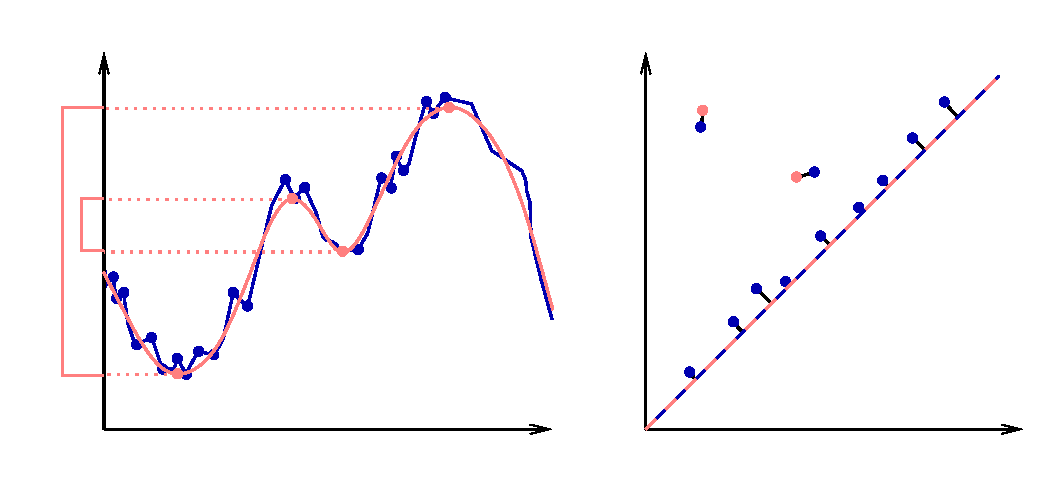
\includegraphics[width=\textwidth,height=0.8\textheight,keepaspectratio]{bottleneck.png}
\end{frame}

\begin{frame}
\frametitle{Bottleneck distance}
\begin{definition}
The bottleneck distance $d_b(\mathcal{A}, \mathcal{B})$ is the smallest $\delta \in \mathbb{R}$ such that there exists a partial matching $\mathcal{A} \longleftrightarrow \mathcal{B}$ where
\begin{itemize}
\item if $a \in \mathcal{A}$ and $b \in \mathcal{B}$ are matched, then $d^\infty(a, b) \leq \delta$;
\item if $a \in \mathcal{A}$ is unmatched, then $d^\infty(a, \Delta) \leq \delta$; and,
\item if $b \in \mathcal{B}$ is unmatched, then $d^\infty(b, \Delta) \leq \delta$; and,
\end{itemize}
\end{definition}
\end{frame}


\begin{frame}
\frametitle{The stability theorem -- Chazal et al. (2009)}

\begin{theorem}
Let $f, g : X \to \mathbb{R}$ be functions on a topological space $X$ and let $\mathbb{U} = H(X^f), \mathbb{V} = H(X^g)$ be the sublevel persistence modules.

If $\mathbb{U}$ and $\mathbb{V}$ are q-tame, then:
\begin{align*}
d_b(\mathsf{dgm}(\mathbb{U}), \mathsf{dgm}(\mathbb{V})) \leq \Vert f - g \Vert_\infty
\end{align*}
\end{theorem}
\end{frame}

\begin{frame}
\nocite{*}
\printbibliography
\end{frame}
\end{document}
